\documentclass[a4paper,12pt]{article}

\usepackage{graphicx}
\usepackage[hidelinks,bookmarks=true]{hyperref}

\renewcommand*{\familydefault}{\sfdefault}
\newcommand{\HRule}{\rule{\linewidth}{0.5mm}}

\begin{document}
\pagenumbering{gobble} 

% Title page
\belowpdfbookmark{Exploring the Effect Of Parallism using Threads}{titlename}
\begin{titlepage}
\begin{center}

% Waikato Uni
\Large University of Waikato\\[1.5cm]
\Large COMP301 - 14B\\[0.5cm]

% Title
\HRule \\[0.4cm] \Large \huge Exploring the Effect Of Parallism using Threads\\[0.4cm] \HRule \\[1.5cm]

% Author
\begin{minipage}{\textwidth}
  \centering
  \emph{Author:} Dan Collins
\end{minipage}

\vfill

% Bottom of the page
{\large \today}

\end{center}
\end{titlepage}

\newpage

\pagenumbering{roman}

% Abstract
\belowpdfbookmark{Abstract}{abstractname}
\begin{abstract}
Modern computers have multiple CPUs which allow programs to run in parallel.
It is possible to use program threads to improve the performance of a single process by exploiting this parallelism.
This project developed a translation program that accepted a compressed (LZ77) input file, made character substitutions and then compressed the output data to a file.
Four different programs were developed with different numbers of threads to see how it effected the process performance.
It was found that splitting the process into an inflation thread and a translation and deflation thread was the best performing.
Splitting the program into three threads where the middle thread needed to wait for both threads to be ready was the worst performing.
\end{abstract}
\newpage

% Contents
\belowpdfbookmark{Contents}{contentsname}
\tableofcontents
\newpage

\pagenumbering{arabic}

%
% Introduction
%
\section{Introduction}
Modern computers make use of multiple CPUs (Central Processing Units) to allow many tasks to happen simultaneously.
This parallelism requires the author of the computer programs to design programs in a way that lets them make use of multiple processors.
Separate programs run as separate processes which allow the operating system to execute programs in parallel and it is possible for a programmer to do this within a single program.
However doing so uses a large memory footprint and communication between processes can be difficult.
Threads are a way of utilising the same methods that facilitate parallelism with processes without needing a larger memory footprint.
The threads making up a program are all defined within a single process which allows them to access shared memory.
Techniques, such as mutexes (Mutual Exclusion), allow the different threads to synchronise and share data.
It is up to the programmer to ensure memory is shared and contention doesn't cause a deadlock.

\section{Method}
A simple translation program was developed to explore the effect of parallelism.
The translation program will accept a compressed file (LZ77), convert some of the symbols, and then compress the output.
Symbols are converted as follows:
\begin{itemize}
  \item All 'a' and 'A' characters must be replaced with '4'.
  \item All 'e' and 'E' characters must be replaced with '3'.
  \item All 'i' and 'I' characters must be replaced with '1'.
  \item All 'o' and 'O' characters must be replaced with '0' (zero).
  \item All 's' and 'S' characters must be replaced with '5'.
\end{itemize}
Four versions were developed to compare how effect threads are.
The control in this experiment is a program with just one main thread.
A program with two threads separates the program into an input thread which decompresses the input file and an output thread which will translate and compress the output data.
A program with three threads has an input thread, a translation thread and an output thread.
This three-thread program performs an in-place translation and then copies the data to an output buffer which is read by the output thread.
Finally, a modification of the three thread program copied data during the translation process.
The code for these programs is attached at the end of this report.
Each program was tested with the same input file three times and a mean time measurement was recorded.
The input files are a random string of characters 'a-z, A-Z' of a specified length.

\section{Results and Discussion}
The program with two threads significantly out performed the others and the program that copied data while translating performed the worst (Fig. 1).

\begin{figure}[h]
  \makebox[\textwidth][c]{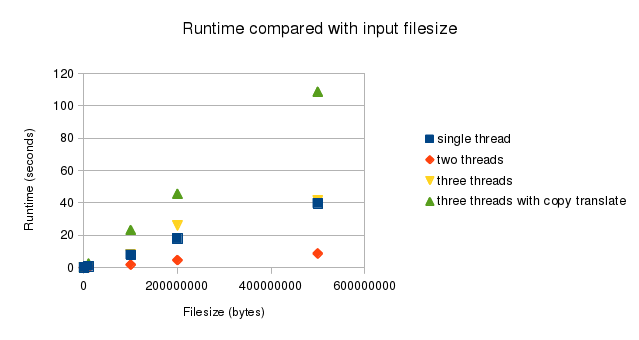
\includegraphics[width=1.2\textwidth]{graph.png}}
  \caption{Runtime Results}
\end{figure}

The results clearly show that care needs to be taken when breaking processes up into threads.
By using too many threads, it is possible to reduce the performance over a simple program with no threads.
The slowest performing program has to wait for both the input and the output thread to have free space in the buffers before it begins the translation process.
The fastest program will inflate data into a buffer in one thread and then translate and deflate data in the other thread.
This experiment did not make use of tools, such as Valgrind, to try measure which parts of the program were running the slowest.
Future work should characterise which parts of the program run the slowest and attempt to optimise those sections, possibly by exploiting parallelism.

\section{Conclusion}
Splitting programs into multiple threads can be an effective way of improving the program's performance.
The threads need to be carefully designed as it is possible to decrease the program performance by using poorly planned threads.


\end{document}
